%%%%%%%%%%%%%%%%%%%%%%%%%%%%%%%%%%%%%%%%%
%
% Reproducible Research Workshop Slides
% Module 01
% Perry Williams
% 09/12/2020
%
%%%%%%%%%%%%%%%%%%%%%%%%%%%%%%%%%%%%%%%%%

% ---------------------------------------------------------
%	PACKAGES AND THEMES
% ---------------------------------------------------------

\documentclass{beamer}\usepackage[]{graphicx}\usepackage[]{color}
% maxwidth is the original width if it is less than linewidth
% otherwise use linewidth (to make sure the graphics do not exceed the margin)
\makeatletter
\def\maxwidth{ %
  \ifdim\Gin@nat@width>\linewidth
    \linewidth
  \else
    \Gin@nat@width
  \fi
}
\makeatother

\definecolor{fgcolor}{rgb}{0.345, 0.345, 0.345}
\newcommand{\hlnum}[1]{\textcolor[rgb]{0.686,0.059,0.569}{#1}}%
\newcommand{\hlstr}[1]{\textcolor[rgb]{0.192,0.494,0.8}{#1}}%
\newcommand{\hlcom}[1]{\textcolor[rgb]{0.678,0.584,0.686}{\textit{#1}}}%
\newcommand{\hlopt}[1]{\textcolor[rgb]{0,0,0}{#1}}%
\newcommand{\hlstd}[1]{\textcolor[rgb]{0.345,0.345,0.345}{#1}}%
\newcommand{\hlkwa}[1]{\textcolor[rgb]{0.161,0.373,0.58}{\textbf{#1}}}%
\newcommand{\hlkwb}[1]{\textcolor[rgb]{0.69,0.353,0.396}{#1}}%
\newcommand{\hlkwc}[1]{\textcolor[rgb]{0.333,0.667,0.333}{#1}}%
\newcommand{\hlkwd}[1]{\textcolor[rgb]{0.737,0.353,0.396}{\textbf{#1}}}%
\let\hlipl\hlkwb

\usepackage{framed}
\makeatletter
\newenvironment{kframe}{%
 \def\at@end@of@kframe{}%
 \ifinner\ifhmode%
  \def\at@end@of@kframe{\end{minipage}}%
  \begin{minipage}{\columnwidth}%
 \fi\fi%
 \def\FrameCommand##1{\hskip\@totalleftmargin \hskip-\fboxsep
 \colorbox{shadecolor}{##1}\hskip-\fboxsep
     % There is no \\@totalrightmargin, so:
     \hskip-\linewidth \hskip-\@totalleftmargin \hskip\columnwidth}%
 \MakeFramed {\advance\hsize-\width
   \@totalleftmargin\z@ \linewidth\hsize
   \@setminipage}}%
 {\par\unskip\endMakeFramed%
 \at@end@of@kframe}
\makeatother

\definecolor{shadecolor}{rgb}{.97, .97, .97}
\definecolor{messagecolor}{rgb}{0, 0, 0}
\definecolor{warningcolor}{rgb}{1, 0, 1}
\definecolor{errorcolor}{rgb}{1, 0, 0}
\newenvironment{knitrout}{}{} % an empty environment to be redefined in TeX

\usepackage{alltt}

\usetheme{Madrid}
\usecolortheme{beaver}

\setbeamertemplate{navigation symbols}{}
\setbeamercolor{block title}{fg=black,bg=darkred}
\setbeamercolor{block body}{fg=black,bg=lightgray}


\usepackage{animate}
\usepackage{booktabs}
\usepackage{graphicx}
\usepackage{mathtools}
\usepackage{mathrsfs}
\usepackage{media9}
\usepackage{listings}
\usepackage{pgf}
\usepackage{stackengine}
\usepackage{textpos}
\usepackage{tikz}
\usepackage{xcolor}
\lstset{breaklines=true} % break long lines
\newcommand\Fontvi{\fontsize{14}{7.2}\selectfont}
\newcommand{\backupbegin}{
  \newcounter{finalframe}
  \setcounter{finalframe}{\value{framenumber}}
}
\newcommand{\backupend}{
  \setcounter{framenumber}{\value{finalframe}}
}
\renewcommand\useanchorwidth{T}
\def\theyearwidth{1.5pt}
\newlength\yrsfboxrule
\yrsfboxrule .4\fboxrule
\newcommand\yearwidth[1]{\def\theyearwidth{#1}\ignorespaces}
\newcommand\skipyears[2][white]{%
  \fboxrule\yrsfboxrule%
  \fboxsep=-\yrsfboxrule%
  \fcolorbox{gray}{#1}{\strut\hspace{#2}}%
  \ignorespaces%
}
\newcommand\showyear[2][black]{%
  \fboxsep=0pt%
  \stackon{%
    \colorbox{#1}{\strut\hspace{\theyearwidth}}
  }{\sffamily\small#2}%
  \ignorespaces%
}

\let\svthefootnote\thefootnote
\textheight 1in
\newcommand\blankfootnote[1]{%
  \let\thefootnote\relax\footnotetext{#1}%
  \let\thefootnote\svthefootnote%
}
\usetikzlibrary{fadings}
\tikzfading[name=fade out, inner color=transparent!0,
         outer color=transparent!100]

\graphicspath{{./Images/}}

% ---------------------------------------------------------
%	TITLE PAGE
% ---------------------------------------------------------

\title[Documentation and reproducibility]{\normalsize Documentation and reproducibility with \texttt{R} and \LaTeX}
\author[Perry Williams]{\footnotesize Perry J. Williams}
\vspace{1in}
\institute[]{
Ecological Statistician\\
  Department of Natural Resources and Environmental Science\\
  University of Nevada, Reno}
\date[09/12/2020]{09/12/2020}

%%%
%%% Begin Document
%%%
\IfFileExists{upquote.sty}{\usepackage{upquote}}{}
\begin{document}

%%%
%%% Make title slide 
%%%

\begin{frame}
\begin{textblock*}{4cm}(8cm,5.8cm) % {block width} (coords)
      \begin{tikzpicture} \path (0,0) rectangle
        (5,7); \node[scope fading=fade out,inner
        sep=0pt,outer sep=0pt,anchor=south east]
        at(5,5)
        {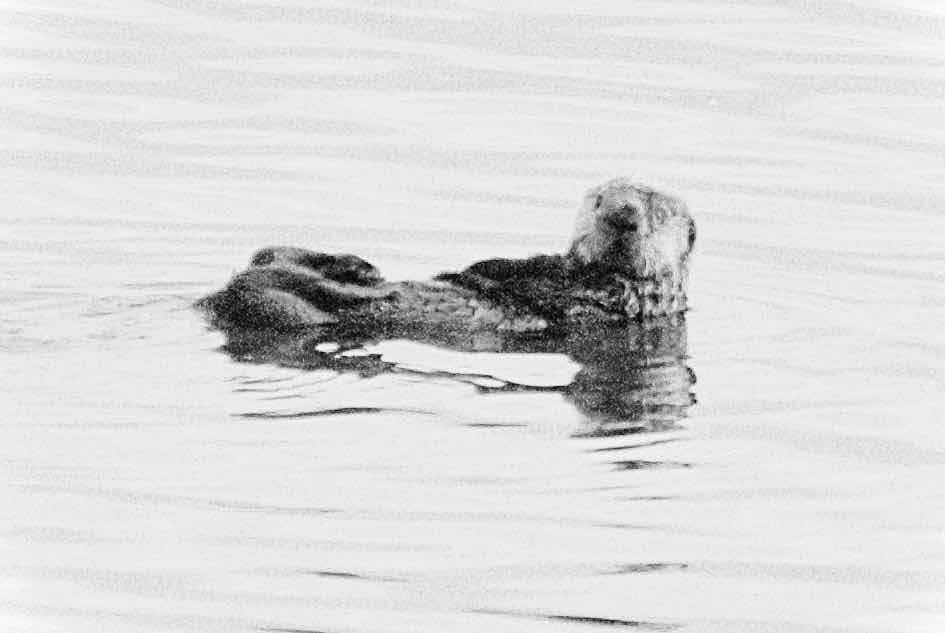
\includegraphics[width=5cm]{icon2}};
      \end{tikzpicture}
  \end{textblock*}
\begin{textblock*}{4cm}(-2cm,5.5cm) % {block width} (coords)
      \begin{tikzpicture} \path (0,0) rectangle
        (5,7); \node[scope fading=fade out,inner
        sep=0pt,outer sep=0pt,anchor=south east]
        at(5,5)
        {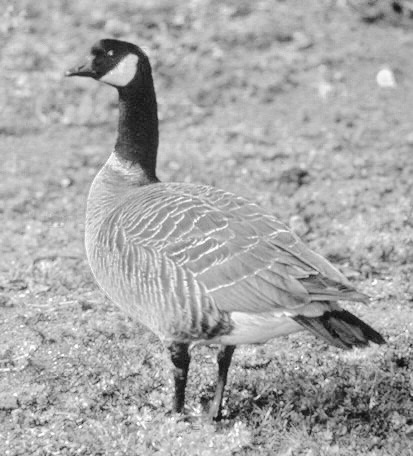
\includegraphics[width=3cm]{cago3}};
      \end{tikzpicture}
  \end{textblock*}
  \titlepage
\end{frame}

% -------------------------------------------------------
% PRESENTATION SLIDES
% -------------------------------------------------------

% ------------------------------------------------
\section{Background \& Motivation}
% ------------------------------------------------

\begin{frame}[noframenumbering]
  \begin{center}
      \textsc{\textrm{Background \& Motivation}}
  \end{center}
\end{frame}


\begin{frame}{Background \& Motivation}
  \begin{center}
    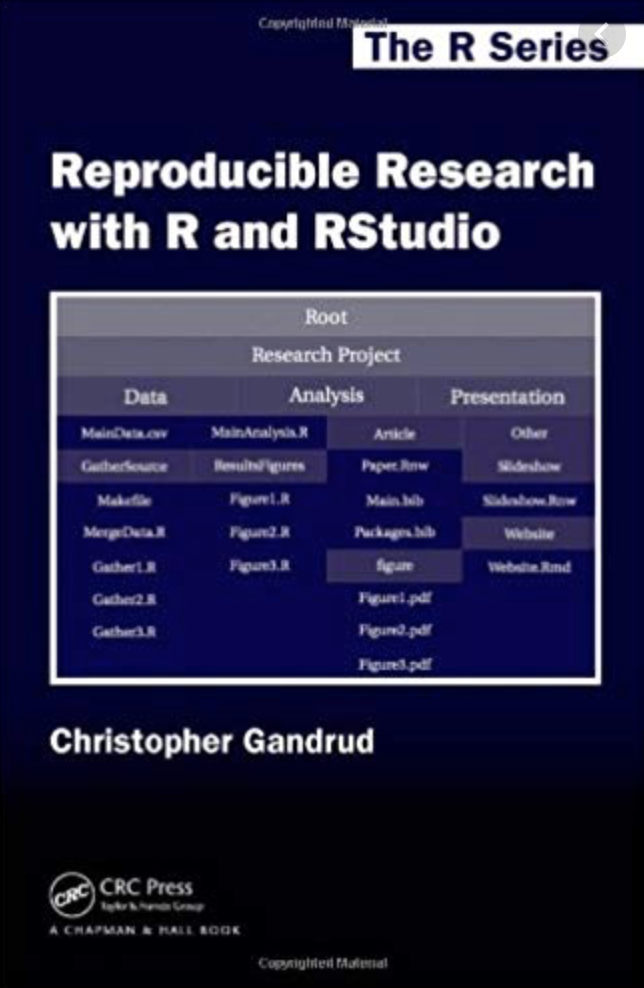
\includegraphics[height=.85\textheight,keepaspectratio]{rr}
  \end{center}
\end{frame}

\begin{frame}[t]{Background \& Motivation}
  \textbf{Research is often presented in very abridged packages}
    \begin{itemize}
      \item Slide shows \vspace{1cm}
      \item Journal articles\vspace{1cm}
      \item Books \vspace{1cm}
      \item Web sites 
    \end{itemize} 
\end{frame}

\begin{frame}[t]{Background \& Motivation}
  \textbf{These presentation documents announce a project's findings}
\end{frame}

\begin{frame}[t]{Background \& Motivation}
  \textbf{These documents are not necissarily the research}
  \begin{itemize}
 \item Sometimes considered the ``advertising" \vspace{1cm}
  \item Especially true in computational and statistical sciences
  \end{itemize}
\end{frame}

\begin{frame}[t]{Background \& Motivation}
  \textbf{The research also includes:}
  \begin{itemize}
    \item Full software environment \vspace{1cm}
    \item Code \vspace{1cm}
    \item Data \vspace{1cm}
  \end{itemize}
\end{frame}

\begin{frame}[t]{Background \& Motivation}
\begin{center}
    
\includegraphics[height=0.8\textheight,keepaspectratio]{finaldoc}
  \end{center}
\end{frame}

\begin{frame}[t]{Background \& Motivation}
   \textbf{This workshop will introduce:}
   \begin{itemize}
\item  The tools to dynamically combine research with presentation of findings,\vspace{.5cm}
     \item The \textbf{\texttt{R}} statistical language for data analysis,\vspace{.5cm}
     \item the \textbf{\LaTeX} mark-up language for documents, slide shows, articles, books, and web-pages,\vspace{.5cm}
     \item the \texttt{knitr} package for \texttt{R},\vspace{.5cm}
     \item \textbf{RStudio}, a program that brings all of these tools together in one place.
   \end{itemize}
 \end{frame}

 \begin{frame}[t]{Objective}
   \textbf{The objective of this workshop is to:}
   \begin{itemize}
      \item   Introduce the tools to develop a work-flow to maximize reproducible-ness, collaborations, and research impact.
      \item Provide templates that can be modified for your own research.\vspace{1cm}
   \end{itemize}
   \textbf{The objective of this workshop is NOT to:}
   \begin{itemize}
      \item Become well-versed in \texttt{R}, \texttt{RStudio}, \texttt{\LaTeX}, or \texttt{knitr} - that takes repetition (starting with the basic building blocks that are provided).
   \end{itemize}
\end{frame}
 
\begin{frame}[t]{Background \& Motivation}
   \textbf{Additional topics include:}
   \begin{itemize}
\item  Version control with Git hub,
     \item Data gathering,
     \item R markdown,
     \item File management,
     \item Projects in RStudio,
     \item Using \LaTeX to make presentations with Beamer.\vspace{1cm} 
   \end{itemize}
   \textbf{All are covered in the book:} \emph{Reproducible Research with R and RStudio}
\end{frame}

 \begin{frame}[t]{Why \texttt{R}?}
  \begin{itemize}
    \item Open Source and free
    \item Very active development community
    \item Interfaces with \LaTeX or other mark-up languages
    \item Explicitly write down analyses steps as source code
   \end{itemize}
 \end{frame}

 \begin{frame}[t]{Why \texttt{knitr}?}
  \begin{itemize}
    \item Literate programming is a crucial part of reproducible quantitative research
    \item Highlights \texttt{R} code in presentation documents making it easier for readers to follow
    \item Provides control over inclusion of graphics
    \item Can cache (save output for later)
   \end{itemize}
 \end{frame}

 \begin{frame}[t]{Why RStudio?}
  \begin{itemize}
    \item Stand alone editor for \TeX  and Markdown
    \item Many shortcuts
    \item Works with C++, CSS, JavaScript, and a few other programming languages
    \item Integrated with version control of Git and SVN
    \item Simple compiling of .Rnw files
    \item \textbf{Easier to learn than Emacs or vi!}
   \end{itemize}
 \end{frame}

% ------------------------------------------------
\section{What is Reproducible Research?}
% ------------------------------------------------

\begin{frame}[t]{What is Reproducible Research?}
     Research results are replicable if there is sufficient information available for independent researchers to make the same findings using the same procedures (King, 1995, 444). \\ \vspace{2cm}
  \only<2->{\textbf{In computational sciences, this means:} \\
  The data and code used to make a finding are available and they are sufficient for an independent researcher to recreate the finding.}
  \end{frame}

\end{document}


